\cotefile{10}
\scanpage{33}
\mspage{\handwritten{1}}
% archive sheet number: 32

\uline{10. Passage à la limite projective dans les préschémas en groupes et les préschémas à groupe d'opérateurs.}

\margin{\handwritten{\figure{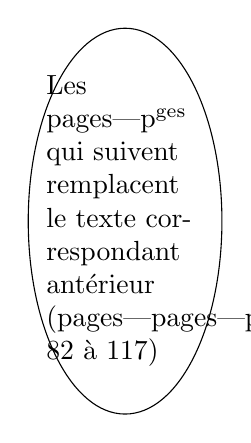
\begin{tikzpicture}
\node[text width=2cm,align=left,inner sep=2pt] at (0,0) {Les \unsure{pages|p\textsuperscript{ges}} qui suivent \unsure{remplacent} le texte correspondant \unsure{antérieur} \unsure{(pages|pages|p\textsuperscript{ges}} 82 à 117)};
\draw (0,0) ellipse (1.23 and 2.45);
\end{tikzpicture}}}}
\handwritten{10.}0. Rappelons le résultat essentiel de (EGA IV 8.8) : Etant donnée la situation suivante : $S_o$ un préschéma qu\handwritten{/}asi-compact et quasi-séparé, $I$ un ensemble préordonné filtrant croissant, $(\handwritten{\unsure{\mathscr{A}|\mathcal{A}}}_i)_{i\handwritten{\in}I}$ un système inductif de $\handwritten{\mathcal{O}}_{S_o}$-Algèbres commutatives quasi-cohérentes, $\handwritten{\mathscr{A}}=\underset{\handwritten{\longrightarrow}}{\lim}\handwritten{\mathscr{A}}_i$, $S_i=\operatorname{Spec}\handwritten{\mathscr{A}}_i$ pour $i\handwritten{\in}I$, et $S=\operatorname{Spec}\handwritten{\mathscr{A}}$, \handwritten{a}lors la catégorie des $S$-préschémas de présentation finie est déterminée à équivalence près par la donnée des catégories des $S_i$-préschémas de présentation finie, des foncteurs \inserted{entre ces catégories} $\handwritten{\rho}_{ij}:X_i\handwritten{\longmapsto}X_i\times_{S_i}S_j$ \deleted{\unsure{,}} pour $i\handwritten{\leqq}j$, et des isomorphismes de transitivité $\handwritten{\rho}_{jk}\mathbin{\unsure{o|\circ}}\handwritten{\rho}_{ij}\handwritten{\xrightarrow{\sim}\rho}_{ik}$. \deleted{Plus précisément,} \handwritten{Précisons.}

\margin{\handwritten{\figure{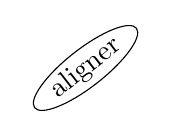
\begin{tikzpicture}
\node[rotate=38,inner sep=1pt] at (0,0) {\unsure{aligner}};
\draw[rotate=38] (0,0) ellipse (.82 and .24);
\end{tikzpicture}}\quad )\quad )}}
Etant donné $j\handwritten{\in}I$, et un $S_j$-préschéma de présentation finie $X_j$, nous poserons,pour tout $i\handwritten{\in}I$ tel que $j\handwritten{\leqq}i$, $X_i=X_j\handwritten{\times}_{S_j}S_i$, et $X=X_j\handwritten{\times}_{S_j}S$. Alors :\inserted{\handwritten{(EGA \uline{IV} 8.8.2)}}\handwritten{\unsure{;|:}}\margin{\handwritten{(}}

\uline{i) Etant donné $j\handwritten{\in}I$, et deux $S_j$-préschémas de présentation finie $X_j$ et $Y_j$, l'application canonique de $\underset{i\handwritten{\geqslant}j}{\underset{\handwritten{\longrightarrow}}{\lim}}\operatorname{Hom} S_i(X_i,Y_i)$ dans $\operatorname{Hom}(X,Y)$ est bijective}\margin{\handwritten{(}}

\uline{ii) Pour tout $S$-préschéma de présentation finie $X$, il existe un indice $j\handwritten{\in}I$, \deleted{et} un $S_j$-préschéma de présentation finie $X_j$ et un $S$-isomorphisme $X\handwritten{\xrightarrow{\sim}}X_j\handwritten{\times}_{S_j}S$.}

On en conclut (EGA IV 8.8.3) que, chaque fois qu'on aura un diagramme $D$ portant sur un nombre fini d'objets et de flèches de la catégorie des $S$-préschémas de présentation finie, on peut trouver un indice $i\handwritten{\in}I$ et un diagramme $D_i$ dans la catégorie des $S_i$-préschémas de présentation finie, tels que le diagramme $D$ provienne à isomorphisme près du diagramme $D_i$ par le changement de base $S\handwritten{\longrightarrow}S_i$. On peut même trouver $i$ et $D_i$ tels que tout carré cartésien de $D$ provienne d'un carré cartésien de $D_i$.

\handwritten{10.1.} De plus, un grand nombre de propriétés \deleted{\unsure{de}} courantes pour un morphisme, stables par changement de base, possèdent la propriété suivante ; étant donné un indice $j\handwritten{\in}I$ deux $S_j$-préschémas de présentation finie $X_j$ et $Y_j$ et un $S_j$-morphisme $u_j:X_j\handwritten{\longrightarrow}Y_j$, pour que $u=u_j\handwritten{\times}_{S_j}S$ ait la propriété $\handwritten{\mathbb{P}}$, il faut et il suffit qu'il existe un indice $i\handwritten{\in}I$ tel que $j\handwritten{\leqq}i$ et que $u_i=u_j\handwritten{\times}_{S_j}S_i$ ait la propriété $\handwritten{\mathbb{P}}$. Il en est ainsi dans le cas où $\handwritten{\mathbb{P}}$ est \deleted{la}\inserted{\handwritten{l'une des}} propriété\inserted{\handwritten{s}}\inserted{\handwritten{suivantes}} pour un morphisme:\deleted{\unsure{d'}}être séparé, surjectif, radiciel, affine, quasi-affine, fini, quasi-fini, propre, projectif, quasi-projectif, un isomor%
\scanpage{34}%
\mspage{\handwritten{2}}%
% archive sheet number: 33
phisme, un monomorphisme, une immersion, une immersion ouverte, une immersion fermée, lisse, non ramifié ou étale (EGA IV 8.10.5, 11.2.6 et 17.7.6). Remarquons qu'il en est encore ainsi \deleted{\unsure{pour}} \uline{dans le cas où $\handwritten{\mathbb{P}}$ est la propriété d'être couvrant pour la topologie \handwritten{\unsure{/|f}}fidèlement plate localement de présentation finie} (notée fppf); en effet, étant donnés deux $S$-préschémas de présentation finie $X$ et $Y$, et un \deleted{morphisme}\inserted{$S$-morphisme} $u:X\handwritten{\longrightarrow}Y$, il résulte de (Exp. IV 6.3.1 (i))\deleted{,} que, pour que $u$ soit couvrant pour la topologie fppf, il faut et il suffit qu'il existe un $S$-préschéma $Z$ et un $S$-morphisme $v:Z\handwritten{\longrightarrow}Y$ fidèlement plat et de présentation finie qui se factorise à travers $u$.

Le but de ce numéro est \deleted{d'étendre}\inserted{\handwritten{de donner des variantes de}} ce genre de résultats \deleted{à}\inserted{\handwritten{pour}} la catégorie des $S$-groupes de présentation finie, \deleted{et à} celle des $S$-préschémas à groupe d'opérateurs, et \deleted{à}\inserted{\handwritten{pour}} certaines propriétés pour des monomorphismes de groupes (être invariant, central, à faisceau quotient inversible, etc ...).

Les deux résultats préliminaires de ce type sont les suivants :

\uline{10.\handwritten{2}.} \deleted{\unsure{a)}} \uline{Dans la situation rappelée au début de (10.0), soient \deleted{\unsure{pour}} $j\handwritten{\in}I$, $G_j$ et $H_j$ deux $S_j$-groupes de présentation finie; posons, pour tout $i\handwritten{\in}I$ tel que $j\handwritten{\leqq}i$, $G_i=G_j\handwritten{\times}_{S_j}S_i$, $G=G_j\handwritten{\times}_{S_j}S$, et définissons de même $\deleted{\unsure{G}}$ $H_i$ et $H$. Alors l'application canonique de $\underset{i\handwritten{\geqslant}j}{\underset{\handwritten{\longrightarrow}}{\lim}}\operatorname{Hom}_{\mathbb{S}_i\text{-gr.}}(G_i,H_i)$ dans $\operatorname{Hom}_{S\text{-gr.}}(G,H)$ est bijective.}

\uline{10.\handwritten{3}.} \deleted{\unsure{b)}} \uline{Dans la situation rappelée au début de (10.0), soit $G$ un $S$-groupe de présentation finie; alors il existe un indice $j\handwritten{\in}I$, \deleted{et} un $S_j$-groupe de présentation \deleted{f} finie $G_j$, et un \deleted{\illegible{1}} $S$-isomorphisme de groupes de $G$ sur $G_j\handwritten{\times}_{S_j}S$.}

Les assertions (10.\handwritten{\unsure{2|1}}) et (10.\handwritten{3}) sont des conséquences faciles de \deleted{(EGA IV 8.8.2 et 8.8.3)}\inserted{\handwritten{(10.0) et (10.1),}} compte tenu de l'interprétation de la structure de $S$-groupe donnée en (EGA $\unsure{0|O}_{\mathrm{III}}$ 8.2.5 et 8.2.6).
\scanpage{35}
\mspage{\handwritten{3}}
% archive sheet number: 34

\deleted{\unsure{fermé} de $H$),}

\deleted{\uline{\unsure{v)|i)} être un monomorphisme central (6.6),}}

\deleted{\uline{vi) être un monomorphisme invariant (6.6).}}

\inserted{\handwritten{10.4.}} \uline{Soient $j\handwritten{\in}I$, $G_j$ et $H_j$ deux $S_j$-groupes de présentation finie, et $u_j:G_j\handwritten{\longrightarrow}H_j$ un morphisme de $S_j$-groupes. Pour que $u=u_j\handwritten{\times}_{S_j}S$ \deleted{ait la propriété $\handwritten{\mathbb{P}}$}\inserted{\handwritten{soit un monomorphisme central (resp. un monomorphisme invariant)}}, il faut et il suffit qu'il existe $i\handwritten{\in}I$, $i\handwritten{\geqslant}j$ tel que $u_i=u_j\handwritten{\times}_{S_j}S_i$ ait la \inserted{\handwritten{même}}propriété $\deleted{\handwritten{\unsure{\mathbb{P}}}}$.}

\deleted{Les assertions (i) à (iv) résultent de (EGA 8.10.5). Les assertions (v) et (vi) sont}\inserted{\handwritten{C'est}} une conséquence immédiate de \deleted{(EGA 8.8.2 et 8.8.3)}\inserted{\handwritten{(10.0) et (10.1),}} compte tenu de la caractérisation donnée en (6.7) des monomorphismes de groupes centraux et invariants.

\inserted{\handwritten{\uline{Corollaire}}} \uuline{10.5.} \uline{Soit $j\handwritten{\in}I$, et soit $G_j$ un $S_j$-groupe de présentation finie. Pour que $G=G_j\handwritten{\times}_{S_j}S$ soit abélien, il faut et il suffit qu'il existe $i\handwritten{\in}I$, $i\handwritten{\geqslant}j$, tel que $G_i=G_j\handwritten{\times}_{S_j}\deleted{\unsure{H}_{\unsure{j|i}}}\inserted{S_i}$ soit abélien.}

En effet, il revient au même de dire qu'un $S$-groupe est abélien, ou que, considéré comme sous-préschéma en groupes de lui-même, il est central.

\uline{Proposition 10.6.}- \uline{Dans la situation rappelée au début de (10.0), soient $j\handwritten{\in}I$, $G_j$ un $S_j$-groupe de présentation finie, $G'_j$ un sous-préschéma en groupes de $G_j$ plat et de présentation finie sur $S_j$. Pour que $G_j\handwritten{\times}_{S_j}S/G'_j\handwritten{\times}_{S_j}S$ soit représentable (pour la topologie fpqc), il faut et il suffit qu'il existe $i\handwritten{\in}I$, $i\handwritten{\geqslant}j$, tel que $G_j\handwritten{\times}_{S_j}S_i/G'_j\handwritten{\times}_{S_j}S_i$ soit représentable.}

C'est une conséquence \deleted{\unsure{p}}du lemme plus général suivant :

\margin{\handwritten{$\mathbb{T}$}}
\uline{Lemme 10.7.}- \uline{Soit $\handwritten{\mathbb{T}}$ la topologie fppf ou fpqc; soient $j\handwritten{\in}I$, $X_j$ un $S_j$-préschéma de}
\scanpage{36}
\mspage{\handwritten{4}}
% archive sheet number: 35
\uline{présentation finie, et $R_j$ une relation d'équivalence sur $X_j$ définie par un $S_j$-monomorphisme $v_j:R_j\handwritten{\longrightarrow}X_j\handwritten{\times}_{S_j}X_j$ tel que le morphisme $\operatorname{pr}_{1,j}\mathbin{\unsure{o|\circ}} v_j:R_j\handwritten{\longrightarrow}X_j$ déduit de $v_j$ par composition avec la première projection $X_j\handwritten{\times}_{S_j}X_j\handwritten{\longrightarrow}X_j$ soit plat et de présentation finie. Alors, pour que le faisceau quotient $X_j\handwritten{\times}_{S_j}S/R_j\handwritten{\times}_{S_j}S$ pour la topologie $\handwritten{\mathbb{T}}$ soit représentable, il faut et il suffit qu'il existe $i\handwritten{\in}I$, $i\handwritten{\geqslant}j$, le faisceau quotient $X_j\handwritten{\times}_{S_j}S_i/R_j{}_{S_j}S_i$ pour la topologie $\handwritten{\mathbb{T}}$ soit représentable.}

Compte tenu des énoncés de (EGA IV 8.8.2, 8.8.3, 8.10.5 et 11.2.6) rappelés en (10.0), ce lemme est conséquence\deleted{\unsure{du}} du résultat suivant :

\uline{Lemme 10.8.}- \uline{Soit $\handwritten{\mathbb{T}}$ la topologie fppf ou fpqc ; soient $\deleted{\unsure{j\in I,}}$ $X$ un $S$-préschéma de présentation finie (resp. localement de présentation finie), $R$ une relation d'\handwritten{é}quivalence sur $X$ définie par un monomorphisme $v:R\handwritten{\longrightarrow}X\handwritten{\times}_S X$ tel que $\operatorname{pr}_1\mathbin{o} v$ soit plat et de présentation finie (resp. plat et localement de présentation finie). Alors les conditions suivantes sont équivalentes :}

\uline{(i) Le faisceau quotient $X/R$ pour la topologie $\handwritten{\mathbb{T}}$ est représentable.}

\uline{(ii) il existe un $S$-préschéma de présentation finie (resp. localement de présentation finie ) $Y$ et un morphisme fidèlement plat $p:X\handwritten{\longrightarrow}Y$ tel que le diagramme}

% Diagram objects and labels typed; connecting arrows handwritten.
\diagram{\(\text{(D)}\)\qquad\begin{tikzcd}[ampersand replacement=\&,column sep=large,row sep=large]
R \handwritten{\arrow[r,"\operatorname{pr}_1\mathbin{o} v"]} \handwritten{\arrow[d,"\operatorname{pr}_2\mathbin{o} v"']} \& X \handwritten{\arrow[d,"p"]} \\
X \handwritten{\arrow[r,"p"']} \& X
\end{tikzcd}}

(où $\operatorname{pr}_1$ et $\operatorname{pr}_2$ sont les projections $X\handwritten{\times}_S X\handwritten{\unsure{\substack{\longrightarrow\\[-.6ex]\rightharpoonup}|\rightrightarrows}}X$) \uline{soit cartésien.}

Notons d'abord que d'après (Exp. IV 3.3.2 et 4.4.3), pour que le faisceau $X/R$ \deleted{\illegible{1}} pour la topologie $\handwritten{\mathbb{T}}$ soit représentable par $Y$, il faut et il suffit que le diagramme (D) soit cartésien et que $p$ soit couvrant pour la topologie $\handwritten{\mathbb{T}}$.

Montrons que i) entraîne ii). L'hypothèse (i) implique que le diagramme (D) est cartésien, donc que $\operatorname{pr}_1\mathbin{o} v$ se déduit de $p$ par changement de base par $p$, et que $p$ est
\scanpage{37}
\mspage{\handwritten{5}}
% archive sheet number: 36
est couvrant pour la topologie fpqc. Puisque $\operatorname{pr}_1\mathbin{\unsure{o|\circ}} v$ est fidèlement plat et de présentation finie, (resp. fidèlement plat et localement \deleted{\unsure{p}}de présentation finie), il en est de même de $p$ (EGA IV 2.7.1), et comme $X$ est de présentation finie (resp. localement de présentation finie) sur $S$, il en est de même de $Y$ (EGA IV 17.7.4).

Montrons que ii) entraîne i). Il suffit de montrer que $p$ est couvrant pour la topologie fppf; or $p$ est fidèlement plat par hypothèse, et localement de présentation finie, puisque $X$ et $Y$ sont localement de présentation finie sur $S$.

\uline{10.9.}- \uline{Dans la situation rappelée au début de (10.0), soient $j\handwritten{\in}I$, et $G_j$ un $S_j$-groupe de présentation finie. Pour que $G^o=(G_j\handwritten{\times}_{S_j}S)^o$ soit représentable, il faut et il suffit qu'il existe \deleted{\unsure{un}} $i\handwritten{\in}I$, $i\handwritten{\geqslant}j$, tel que $(G_i)^o=(G_j\handwritten{\times}_{S_j}S_i)^o$ soit représentable.}

La condition est suffisante (3.3).

Montrons que la condition est nécessaire. \deleted{Alors}\inserted{\handwritten{En effet,}} $G^o$ est de présentation finie sur $S$ et ouvert dans $G$ (3.9). D'après (10.0), il existe $i\handwritten{\in}I$, $i\handwritten{\geqslant}j$, et un sous-préschéma en groupes ouvert $G_i^o$ de $G_i$ tel que $G_i^o\handwritten{\times}_{S_i}S=G^o$. Le morphisme structural $G^o\handwritten{\longrightarrow}S$ est connexe (i.e. à fibres géométriquement connexes)(Exp. $\mathrm{VI}_A$ 2.1.1). Alors, (EGA IV 9.3.3 et 9.7.7), quitte à augmenter $i$, on peut supposer que le morphisme structural $G_i^o\handwritten{\longrightarrow}S$ est connexe, donc que l'espace sous-jacent à $G_i^o$ n'est autre que \uline{$\handwritten{(}G_i^{\deleted{o}}\handwritten{)^o}$} (3.10.1), donc que $G_i^o$ représente $(G_i)^o$.

\uline{10.10.} \uuline{Rappelons deux cas particuliers très utiles de la situation énoncée en (10.0)}

a) Etant donné un point $x$ d'un préschéma $X$, on pose $S_o=\operatorname{Spec}\handwritten{\mathbb{Z}}$\handwritten{/}et on considère la famille $(S_i)_{i\handwritten{\in}I}$ filtrante décroissante des voisinages \deleted{\unsure{principaux}} ouverts affines de $x$; alors $S=\operatorname{Spec}\handwritten{\mathcal{O}}_{X,x}$. En particulier, si $x$ est le point générique d'un schéma intègre $X$, on trouve $S=\handwritten{\kappa}(x)$.

b) On pose $S_o=\operatorname{Spec}\handwritten{\mathbb{Z}}$, et on considère la famille $(\handwritten{\unsure{\mathscr{A}|\mathcal{A}}}_i)_{i\handwritten{\in}I}$ préordonnée par inclusion des sous-$\handwritten{\mathbb{Z}}$-algèbres de type fini de l'anneau d'un schéma affine $S$.
\scanpage{38}
\mspage{\handwritten{6}}
% archive sheet number: 37

\margin{\handwritten{\figure{
\begin{tikzpicture}[scale=.75]
\node[rotate=25,inner sep=1pt] at (0,0) {intervertir};
\draw[rotate=25] (0,0) ellipse (1.05 and .27);
\end{tikzpicture}}}}
Etant donné que les $\handwritten{\unsure{\mathscr{A}|\mathcal{A}}}_i$ sont des anneaux \deleted{\unsure{pas}} \unsure{nœ thériens|nœthériens}, cela permet dans de nombreux\inserted{\handwritten{cas}} de passer
% The typed words retain their positions; the circles and transposition arrow are handwritten.
\figure{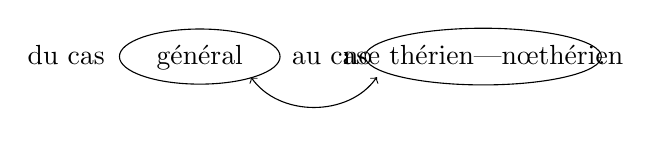
\begin{tikzpicture}
\node[anchor=base east,inner sep=0pt] at (-1.2,0) {du cas};
\node[anchor=base,inner sep=0pt] at (0,0) {général};
\node[anchor=base,inner sep=0pt] at (1.65,0) {au cas};
\node[anchor=base,inner sep=0pt] at (3.6,0) {\unsure{nœ thérien|nœthérien}};
\node[anchor=base west,inner sep=0pt] at (5.05,0) {.};
\handwritten{\draw (0,.10) ellipse (1.02 and .35);
\draw (3.6,.10) ellipse (1.50 and .36);
\draw[<->] (.65,-.16) to[out=-55,in=-125] (2.25,-.16);}
\end{tikzpicture}}

Nous allons maintenant donner deux résultats concernant le cas particulier envisagé en a).

\uline{Proposition 10.11.}- \uline{Soient $S$ un préschéma intègre de point générique $\handwritten{\eta}$, $G$ un $S$-groupe de présentation finie, $X$ un $S$-préschéma de présentation finie, $u$ et $v$ deux $S$-morphismes de $X$ dans $G$, $i:H\handwritten{\longrightarrow}G$ et $j:K\handwritten{\longrightarrow}G$ deux monomorphismes de présentation finie. Alors :}

\uline{(i) il existe un ouvert non vide $S'$ de $S$ tel que si on note $G'$ (resp $H'$, resp. $X'$, resp $u'$, resp $v'$) la restriction de $G$(resp. $H$,resp. $X$, resp. $u$,resp. $v$) au-dessus de l'ouvert $S'$ de $S$, le foncteur\deleted{\unsure{s}} $\underline{\operatorname{Transp}}(u',v')$ (resp. $\underline{\operatorname{Centr}}(u')$, $\underline{\operatorname{Centr}}_{G'}H')$ soit représentable par un sous-$S'$-préschéma fermé de présentation finie $T'_1$ (resp. $C'_1$, resp. $C'_2$) de $G'$.}

\uline{(ii) supposons que $K_{\handwritten{\eta}}$ soit fermé dans $G_{\handwritten{\eta}}$ (ce qui est le cas si $K$ est un sous-$\deleted{\unsure{p}}S$-préschéma en groupes de $G$ (1.4.2)); alors il existe un ouvert non vide $S'$ de $S$ tel que si on note $G'$ (resp. $H'$, resp. $K'$) la restriction de $G$ (resp. $H$, resp. $K$)au-dessus de l'ouvert $S'$ de $S$, le foncteur $\underline{\operatorname{Transp}}_{G'}(H',K')$ (resp. $\underline{\operatorname{Norm}}_{G'}K')$ soit représentable par un sous-$S'$-préschéma fermé de présentation finie $T'_2$ (resp. $N'$) de $G'$.}

\uline{(iii)supposons que $H_{\handwritten{\eta}}$ et $K_{\handwritten{\eta}}$ soient fermés dans $G_{\handwritten{\eta}}$ (ce qui est le cas si $H$ et $K$ sont des sous-préschémas en groupes de $G$ (1.4.2)); alors il existe \inserted{\handwritten{un ouvert}} non vide $S'$ de $S$ tel que si on note $G'$ (resp $H'$, resp. $K'$) la restriction de $G$ (resp. $H$, resp. $K$) au-dessus de l'ouvert $S'$ de $S$, le foncteur $\underline{\operatorname{Transpstr}}_{G'}(H',K')$ soit représentable par un sous-$S'$-préschéma fermé de présentation finie de $G'$.}

Puisque $G_{\handwritten{\eta}}$, $X_{\handwritten{\eta}}$, $H_{\handwritten{\eta}}$, $K_{\handwritten{\eta}}$ sont plats sur le corps $\handwritten{\kappa}(\handwritten{\eta})$, et que
\scanpage{39}
\mspage{\handwritten{7}}
% archive sheet number: 38
$G_{\handwritten{\eta}}$ est séparé sur $\handwritten{\kappa}(\handwritten{\eta})$ (\deleted{Exp.} $\mathrm{VI}_A$ 0.2), d'après (10.2,10.10 a),EGA IV 8.8.2 et 8.10.5), il existe un ouvert\inserted{affine} $S'$ de $S$ tel que $G'$ soit un $S'$-groupe de \deleted{type}\inserted{présentation} fini, plat et séparé sur $S'$, et que $X'$, $H'$ et $K'$ soient plats et de présentation finie sur $S'$. Si on suppose $H_{\handwritten{\eta}}$ (resp. $K_{\handwritten{\eta}}$) fermé dans $G_{\handwritten{\eta}}$, on peut choisir $S'$ de sorte que $H'$ (resp. $K'$) soit fermé dans $G'$. D'après (EGA IV 11.3.15), quitte à remplacer $S'$ par un ouvert affine de $S'$, on peut supposer que $G'$, $H'$, $K'$ et $X'$ sont essentiellement libres sur $S'$ (au sens de \deleted{Exp.} VIII (6.1)). Il résulte alors de (\deleted{Exp.} VIII \handwritten{5}.5 b) et e)\textsuperscript{(*)}) que, sous les hypothèses de l'énoncé, les foncteurs considérés sont représentables par des sous-préschémas fermés (donc de présentation finie sur $S'$) de $G'$.

\uline{Proposition 10.12.- Soient $S$ un préschéma intègre, $G$ un \deleted{$S$-préschéma} $S$-groupe de présentation finie, $A$ et $B$ deux sous-préschémas en groupes de présentation finie de $G$, à fibre générique lisse, tels que \deleted{ou bien $A$ soit à fibres connexes}\inserted{$A$ soit à fibre générique connexe}, \deleted{ou \unsure{bien bien|bien}}\inserted{(resp.} $A$ et $B$ soient invariants dans $G$). Alors il existe un ouvert non vide $S'$ de $S$ et un sous-préschéma en groupes\inserted{\handwritten{fermé, $D'$}} de présentation finie, à fibres lisses \deleted{et fermé $D'$} de $G'=G\handwritten{|}S'$\handwritten{,} tel que $D'$ soit \deleted{co} à fibres connexes (resp. soit invariant dans $G'$), et que $D'$ représente le faisceau associé, pour la topologie fppf ou fpqc, au préfaisceau en groupes des commutateurs de $A$ et $B$ dans $G$. En particulier, pour tout $s\handwritten{\in}S'$, on a $D'_s=(A_s,B_s)$ avec les notations de (7.2 (vii)).}

Soit $\handwritten{\eta}$ le point générique de $S$; posons $D'_{\handwritten{\eta}}=(A_{\handwritten{\eta}},B_{\handwritten{\eta}})$. D'après (7.8) (resp. 7.3 v)), $D'_{\handwritten{\eta}}$ est connexe (resp. invariant dans $G_{\handwritten{\eta}}$). D'après (10.1 et 10.10 a)), il existe un ouvert non vide $S'$ de $S$ et un sous-$S'$-préschéma en groupes $D'$ de présentation finie et fermé dans $G'$, à fibres séparables (EGA IV 9.7.7 et 9.3.3), ayant $D'_{\handwritten{\eta}}$ pour fibre au point $\handwritten{\eta}$, et tel que $D'$ soit à fibres connexes (i.e. géométriquement connexes (\deleted{Exp.} $\mathrm{VI}_A$ 2.1.1))(resp. soit invariant dans $G'$)(EGA IV 9.7.7 et 9.3.3\inserted{\handwritten{)}}(resp. (10.4)). De plus, nous avons vu, au cours de la démonstration de (7.8), qu'il existe un entier $n$ tel que $\handwritten{\unsure{\gamma|\upsilon}}_{\handwritten{\eta}}^n((A_{\handwritten{\eta}}\times_{\handwritten{\kappa}(\handwritten{\eta})}B_{\handwritten{\eta}})^n)=D'$, où $\handwritten{\gamma}_{\handwritten{\eta}}:A_{\handwritten{\eta}}\times_{\handwritten{\kappa}(\handwritten{\eta})}B_{\handwritten{\eta}}\handwritten{\longrightarrow}G_{\handwritten{\eta}}$

\par\noindent\handwritten{\rule{\linewidth}{0.3pt}}\par
\handwritten{(*) Voir note page 51 \textcircled{\unsure{40|10}}}\par
\scanpage{40}
\mspage{\handwritten{8}}
% archive sheet number: 39
est défini comme en (7.2 (vii)). Nous pouvons définir, par les mêmes formules qu'en (7.2 (vii)et 7.1 (ii)), les morphismes $\handwritten{\unsure{\gamma|\upsilon}}':A'\handwritten{\times}_{S'}B'\handwritten{\longrightarrow}G'$ et $\handwritten{\gamma}'^n:(A'\handwritten{\times}_{S'}B')^n\handwritten{\longrightarrow}G'$, on a bien $\handwritten{\gamma}'^n_{(\handwritten{\kappa}(\handwritten{\eta}))}=\handwritten{\gamma}^n_{\handwritten{\eta}}$. Par conséquent (EGA IV 8.8.3 et 8.10.5\deleted{)}\inserted{et 11.2.6)}\handwritten{,} on peut choisir $S'$ tel que le morphisme $\handwritten{\gamma}'^n$\inserted{soit plat \handwritten{et}} se factorise à travers $D'$, et que le morphisme $(A'\handwritten{\times}_{S'}B')^n\handwritten{\longrightarrow}D'$ déduit de $\handwritten{\gamma}'^n$ soit surjectif. Alors (7.5) le morphisme $(A'\handwritten{\times}_{S'}B')^{n+1}\handwritten{\longrightarrow}D'$ déduit de $\handwritten{\gamma}'^{n+1}$ est couvrant pour la topologie fppf (et a fortiori pour la topologie fpqc). Donc $D'$ représente le faisceau associé,pour la topologie fppf ou fpqc, au préfaisceau des commutateurs de $A$ et $B$ dans $G$. De plus, pour tout $s\handwritten{\in}S'$, le morphisme $(A_s\handwritten{\times}_{\handwritten{\kappa}(s)}B_s)^n\handwritten{\longrightarrow}D'_s$ déduit de $\handwritten{\gamma}^n_s$ est surjectif; donc (7.6), $(A_s,B_s)$ représente le faisceau des commutateurs de $A_s$ et $B_s$ dans $G_s$ (pour la topologie fppf ou fpqc), d'où $D'_s=(A_s,B_s)$.

\uline{Corollaire 10.1\handwritten{3}.}- \uline{Soient $S$ un préschéma intègre de point générique $\handwritten{\eta}$, $G$ un $S$-groupe de présentation finie, $D$ un sous-$S$-préschéma en groupes de présentation finie de $G$ à fibres lisses et invariant dans $G$. Supposons qu'on ait $(D_{\handwritten{\eta}},D_{\handwritten{\eta}})=D_{\handwritten{\eta}}$ (resp. $(G_{\handwritten{\eta}},D_{\handwritten{\eta}})=D_{\handwritten{\eta}}$). Il existe alors un ouvert non vide $S'$ de $S$ tel que pour tout $s\handwritten{\in}S'$, on ait $(D_s,D_s)=D_s$ (resp. $(G_s,D_{\handwritten{\unsure{e|s}}})=D_s$).}

Cela résulte immédiatement de (10.12) et de (EGA IV 8.8.2.5).

Les énoncés (10.\handwritten{2}) et (10.\handwritten{3}) concernant la catégorie des $S$-groupes de présentation finie\handwritten{[}s'étendent à la catégorie des couples formés d'un $S$-groupe de présentation finie et d'un \deleted{préschéma} $S$-préschéma de présentation finie à groupe d'opérateurs $G$. De façon précise :

\uuline{10.14.} \uline{(i) Dans la situation rappelée au début de (10.0), soient $j\handwritten{\in}I$, $G_j$ et $G'_j$ deux $S_j$-groupes de présentation finie, $H_j$(resp. $H'_j$) un $S_j$-préschéma de présentation}
\scanpage{41}
\mspage{\handwritten{9}}
% archive sheet number: 40
finie à groupe d'opérateurs $G_j$ (resp. $G'_j$). Posons, pour $i\handwritten{\in}I$, $i\handwritten{>}j$, $G_i=G_j\handwritten{\times}_{S_j}S_i$ et $G=G_j\handwritten{\times}_{S_j}S$, et définissons de même $G'_i$, $G'$, $H_i$,$H$, $H'_i$, et $H'$. Notons $\operatorname{Dihom}_{S\text{-gr.}}((G,\handwritten{\unsure{H|H'|\mathbb{H}|\mathbb{H}'}}),(\handwritten{\unsure{G|\mathbb{G}}}',H'))$ l'ensemble des di-morphismes de $S$-groupes et de $S$-préschémas à groupe d'opérateurs du couple $(G,H)$ dans le couple $(G',H')$. Alors l'application canonique de $\underset{i\handwritten{>}j}{\underset{\handwritten{\longrightarrow}}{\lim}}{\mathbb{D}\mathrm{ihom}}_{S_i\text{-gr.}}((G_i,H_i),(G'_i,H'_i))$ dans $\operatorname{Dihom}_{S\text{-gr.}}((G,H),(G',H'))$ est bijective.

(ii) Dans la situation rappelée au début de (10.0), soient $G$ un $S$-groupe \deleted{\unsure{fini}} de présentation finie et $H$ un $S$-préschéma de présentation finie à groupe d'opérateurs $G$; il existe alors un indice $j\handwritten{\in}J$, un $S_j$-groupe de présentation finie $G_j$, un $S_j$-préschéma de présentation finie $H_j$ à groupe d'opérateurs $G_j$ et un di-isomorphisme de $S$-groupes et de $S$-préschémas à groupes d'opérateurs de $(G_j\handwritten{\times}_{S_j}S,H_j\handwritten{\times}_{S_j}S)$ sur$(G,H)$

\deleted{Proposition}\inserted{Définition} 10.15.- Etant donné un $S$-foncteur enngroupes $G$ et un $S$-foncteur $H$ à groupe d'opérate$\overset{\handwritten{\curvearrowleft}}{\underset{\handwritten{\curvearrowright}}{\mathrm{ru}}}$s $G$, on dit que $H$ est un \uline{$S$-foncteur en espaces homogènes sous $G$ pour la topologie $\handwritten{\mathbb{T}}$}, si le morphisme canonique $G\handwritten{\times}_S H\handwritten{\longrightarrow}H\handwritten{\times}_S H$ (défini par $(g,h)\handwritten{\longmapsto}(g.h,h)$ pour $g\handwritten{\in}G(T)$, $h\handwritten{\in}H(T)$) est un épimorphisme de faisceaux pour la topologie $\handwritten{\mathbb{T}}$.

Si $G$ est un $S$-groupe et si $H$ est un $S$-préschéma à \deleted{groupe} groupe d'opérateurs $G$, dire que $H$ est un $S$-préschéma en espaces homogènes sous $G$ pour la topologie $\handwritten{\mathbb{T}}$ revient donc à dire que le morphisme canonique $G\handwritten{\times}_S H\handwritten{\longrightarrow}H\handwritten{\times}_S H$ défini comme précédemment est couvrant pour la topologie $\handwritten{\mathbb{T}}$ (\deleted{Exp.} IV 4.4.3).

De même, dire qu'un $S$-préschéma $H$ à groupe d'opérateurs un $S$-groupe $G$ est un fibré principal homogène sous $G$ pour la topologie $\handwritten{\mathbb{T}}$ (\deleted{Exp.} IV 5.1.5) revient à dire (\deleted{Exp.} IV 5.6 (ii)) que le morphisme canonique $G\handwritten{\times}_S H\handwritten{\longrightarrow}H\handwritten{\times}_S H$ est un isomorphisme et que le morphisme structural $H\handwritten{\longrightarrow}S$ est couvrant pour la topologie $\handwritten{\mathbb{T}}$.

\uline{10.16.- Dans la situation rappelée au début de (10.0) , soient $j\handwritten{\in}I$, $G_j$ un $S_j$-grou-}
% The final word continues beyond the supplied scans.
